%!TEX program = xelatex
\documentclass[10pt,xcolor={x11names}]{beamer}

\usepackage{amsmath, latexsym, amssymb, url, amssymb, pgfplots, amsthm, mathtools, setspace, commath, tikz, verbatim, array, bbding, bigints, fontspec, xunicode, xltxtra, geometry, algorithm, algpseudocode, graphicx, listings, lipsum, tabto, tcolorbox, booktabs, siunitx, caption, float}

\usetheme{B}

\newfontfamily\Codefont{Courier}  %{GillSans} %{AmericanTypewriter}

\definecolor{gry}{rgb}{1,1,1}

\lstset{language=C++,
                moredelim=[is][\color{Green3}\Codefont]{<}{>},
                basicstyle=\small\Codefont,
                identifierstyle=\Codefont,
                directivestyle=\color{Coral1}\Codefont,
                keywordstyle=\color{DeepPink2}\Codefont,
                stringstyle=\color{SeaGreen4}\Codefont,
                commentstyle=\color{Snow4}\Codefont,
                emphstyle=\color{DeepSkyBlue3}\Codefont,
                emph={double,int,float,void,long},
                showspaces=false,
                %keywordstyle=[2]\color{Violet},
                keywords=[2]{*,1,2,3,4,5,6,7,8,9,0},
                keywordstyle=[2]\color{blue},
                showstringspaces=false,
                morecomment=[l][\color{orange}]{\#}}
\lstset{literate=%
    *{0}{{{\color{DarkOrchid3}0}}}1
    {1}{{{\color{DarkOrchid3}1}}}1
    {2}{{{\color{DarkOrchid3}2}}}1
    {3}{{{\color{DarkOrchid3}3}}}1
    {4}{{{\color{DarkOrchid3}4}}}1
    {5}{{{\color{DarkOrchid3}5}}}1
    {6}{{{\color{DarkOrchid3}6}}}1
    {7}{{{\color{DarkOrchid3}7}}}1
    {8}{{{\color{DarkOrchid3}8}}}1
    {9}{{{\color{DarkOrchid3}9}}}1
    {.0}{{{\color{DarkOrchid3}.0}}}2
    {.1}{{{\color{DarkOrchid3}.1}}}2
    {.2}{{{\color{DarkOrchid3}.2}}}2
    {.3}{{{\color{DarkOrchid3}.3}}}2
    {.4}{{{\color{DarkOrchid3}.4}}}2
    {.5}{{{\color{DarkOrchid3}.5}}}2
    {.6}{{{\color{DarkOrchid3}.6}}}2
    {.7}{{{\color{DarkOrchid3}.7}}}2
    {.8}{{{\color{DarkOrchid3}.8}}}2
    {.9}{{{\color{DarkOrchid3}.9}}}2
}
\lstset{alsolanguage=[90]Fortran}
\lstset{alsolanguage=python}
\lstset{backgroundcolor=\color{gry}}
\lstset{frame=single}
\lstset{
    numbers=left,
    numberstyle=\Codefont,
    tabsize=4,
}

\title{Schr\"{o}dinger's Equation}
\subtitle{Two Electrons in a 3D Harmonic Oscillator Well}
\author{Thomas Bolden}
\date{2016}

\setcounter{showSlideNumbers}{1}

\begin{document}

	\setcounter{showProgressBar}{0}
	\setcounter{showSlideNumbers}{0}

	\frame{\titlepage}

	\begin{frame}
		\frametitle{Contents}
		\begin{enumerate}
			\item Introduction
			\item Methods - Theory and Algorithms
			\item Results
			\item Conclusions
			\item Summary
		\end{enumerate}
	\end{frame}

	\setcounter{framenumber}{0}
	\setcounter{showProgressBar}{1}
	\setcounter{showSlideNumbers}{1}

	\section{Introduction}

		\begin{frame} \frametitle{Why? {\em The Background}}
			The Schr\"{o}dinger equation for one confined electron is a relatively simple example of a particle in a potential well. The two-electron case however, becomes much more challenging due to the repulsive interaction between the electrons.

			This means we really want a numerical solution!
		\end{frame}

		\begin{frame}
			\frametitle{Why? {\em The Motivation}}
			\begin{itemize}
				\item<1-> Schr\"{o}dinger's equation is difficult to solve analytically
				\item<2-> Numerical methods work on more complex systems
				\item<3-> Computational methods are adaptable
			\end{itemize}
		\end{frame}

		\begin{frame} \frametitle{The Process}
			Two methods of computing eigenvalues of a matrix were implimented and compared: 
			Jacobi rotation and Armadillo's {\em eig\_sym}
			Since the one-electron solution is simple to solve analytically, it provides a reasonable standard to check the algorithms. 
		\end{frame}

	\section{Methods}

		\begin{frame}
			\frametitle{The Single Electron Case}
			The radial Schr\"{o}dinger equation for one electron is given by
			\[ -\dfrac{\hbar^2}{2m} \left( \dfrac{1}{r^2} \dfrac{d}{dr}r^2\dfrac{d}{dr} - \dfrac{\ell (\ell -1)}{r^2} \right) R(r) + V(r) R(r) = E R(r) \;\; , \;\; V(r) = \dfrac{m\omega^2 r^2}{2} \]
			The energy solutions can be quantized
			\[ E_{nl} = \hbar \omega \left( 2n+l+\dfrac{3}{2} \right) \]
			This is not yet helpful!
		\end{frame}

		\begin{frame} \frametitle{The Single Electron Case}
			If, in spherical coordinates, a dimensionless variable is introduced such that $\rho = r/\alpha$, with $\alpha$ having dimensions of length, the equation becomes
			\[ -\dfrac{\hbar^2}{2m\alpha^2} \dfrac{d^2}{d\rho^2} u(\rho) + \left( V(\rho) + \dfrac{l(l+1)}{\rho^2} \dfrac{\hbar^2}{2m\alpha^2} \right) u(\rho) = Eu(\rho). \]
			If we neglect angular momentum by setting $l=0$, and making $\omega = \alpha \rho$, we get
    		\[ -\dfrac{\hbar^2}{2m\alpha^2} \dfrac{d^2}{d\rho^2} u(\rho) + \dfrac{k}{2} \alpha^2 \rho^2 u(\rho) = Eu(\rho) \]
		\end{frame}

		\begin{frame} \frametitle{The Single Electron Case}
			If both sides of the previous equation are multiplied by $\dfrac{2m\alpha^2}{\hbar^2}$ while fixing $\alpha = \left( \dfrac{\hbar^2}{mk} \right)^{1/4}$ the equation becomes
    		\[ -\dfrac{d^2}{d\rho^2} u(\rho)+ \rho^2 u(\rho) = \lambda u(\rho). \]
    		Discrete energy eigenvalues are given by
    		\[ \lambda = \dfrac{2m\alpha^2}{\hbar^2}. \]
    		The first three eigenvalues are therefore $\lambda_0 = 3$, $\lambda_1 = 7$, $\lambda_2 = 11$. 
		\end{frame}

		\begin{frame} \frametitle{The Single Electron Case}
			In order to solve this, the standard approximation of the second derivatve with step length $h$ will be used.
    		\[ u'' = \dfrac{u(\rho+h)-2u(\rho)+u(\rho-h)}{h^2} + O(h^2) , \]
    		If we let 
    		\begin{align*}
    			u_i &= u(\rho)\\
    			u_{i\pm 1} &= u(\rho \pm h) \\
    			\rho_i &= ih \\
    			V_i &= V(\rho_i)
    		\end{align*}
    		we can discretize the second derivative to
    		\[ -\dfrac{u_{i+1} + u_{i-1} - 2u_i}{h^2} + V_i u_i = \lambda u_i \]
		\end{frame}

		\begin{frame} \frametitle{The Single Electron Case}
			The previous equation resembles a set of linear equations.
			The finial tridiagonal matrix which is the solution to \textbf{Au} = $\lambda$\textbf{u} is then
    		\[ \textbf{A} = 
    		\left( \begin{array}{cccccc} 
    		\frac{2}{h^2}+V_1 & -\frac{1}{h^2}   & 0    & \dots  &0     & 0 \\
   		 	-\frac{1}{h^2} & \frac{2}{h^2}+V_2 &  -\frac{1}{h^2}   & \dots  &0     &0 \\
    		0   & -\frac{1}{h^2} &  \cdots  & \dots      &\dots & 0\\
    		\dots  & \dots  & \dots  &\dots      &\dots & \dots\\
    		0   & \dots & \dots  &\dots       &\frac{2}{h^2}+V_{n{-2}} & -\frac{1}{h^2}\\
    		0   & \dots & \dots  &\dots       &-\frac{1}{h^2} & \frac{2}{h^2}+V_{n-1}
    		\end{array} \right)  
    		\]
    		with \textbf{u} = $(u_1 \; u_2 \; \dots \; u_{n-1})^T$
		\end{frame}

		\begin{frame} \frametitle{The Single Electron Case}
			Now that I have shown how the Schr\"{o}dinger equation can be written as a set of linear equations, I can now talk about how it might be solved computationally.
		\end{frame}

		\begin{frame} \frametitle{Jacobi's Rotation Algorithm}
			This linear equation solver uses a rotation matrix to solve for the eigenvalues of \textbf{A}. Given a square matrix, Jacobi's algorithm rotates the matrix until only the only remaining non-zero elemets in the matrix exist on the diagonal. These numbers are the eigenvalues.
		\end{frame}

		\begin{frame} \frametitle{Jacobi's Rotation Algorithm}
			The first step in Jacobi's algorithm is finding the largest off-diagonal element in the matrix. This is implemented in the code that follows.
		\end{frame}

		\begin{frame} \frametitle{Jacobi's Method in C++ Code}
			\lstinputlisting[language=C++]{Code/MaxOffDiagonal.cpp}
		\end{frame}

		\begin{frame} \frametitle{Jacobi's Rotation Algorithm}
			Once the largest off-diagonal matrix element is found, the rotation matrix \textbf{R}  (the standard sine, cosine rotation matrix) can be applied to \textbf{A}.
			\centerline{\textbf{B} = \textbf{R}$^T$\textbf{AR}}
			The elements of \textbf{B} are equations involving $\sin \theta$ and $\cos \theta$.
			\begin{align*}
  			B_{ik} =& A_{ik}\cos\theta - A_{il}\sin\theta , i \ne k, i \ne l \\
  			B_{il} =& A_{il}\cos\theta + A_{ik}\sin\theta , i \ne k, i \ne l \\
  			B_{kk} =& A_{kk}\cos^2\theta - 2A_{kl}\cos\theta \sin\theta +A_{ll}\sin^2\theta\\
  			B_{ll} =& A_{ll}\cos^2\theta +2A_{kl}\cos\theta sin\theta +A_{kk}\sin^2\theta\\
  			B_{kl} =& (A_{kk}-A_{ll})\cos\theta \sin\theta +A_{kl}(\cos^2\theta-\sin^2\theta)
			\end{align*}
			The following slides show this implemented in C++.
		\end{frame}

		\begin{frame} \frametitle{Jacobi's Rotation in C++}
			\lstinputlisting[language=C++]{Code/RotateA.cpp}
		\end{frame}

		\begin{frame} \frametitle{Jacobi's Rotation in C++}
			\lstinputlisting[language=C++]{Code/RotateB.cpp}
		\end{frame}

		\begin{frame} \frametitle{Jacobi's Rotation in C++}
			\lstinputlisting[language=C++]{Code/RotateC.cpp}
		\end{frame}

	\section{Results}
		\begin{frame} \frametitle{Evaluating $\; \rho \;$ Dependency}
			When the dimensionality of the matrix is changed, the  dimensionless variable $\rho$ needed to accurately determine the lowest three eigenvectors also changes.
    		\[
    		\begin{array}{cc}
    		\toprule \midrule
     		\text{Minimum } \rho_\text{max} & \text{Matrix Dimensions } n  \\ \midrule
    		5 & 200 \\ \midrule
    		6 & 250 \\ \midrule
    		7 & 300 \\ \midrule
    		8 & 350 \\ \midrule
    		9 & 400 \\ \midrule
    		10 & 450 \\ \midrule
    		\bottomrule
    		\end{array}
    		\]
    		% say something about the 4 leading digits
		\end{frame}

		\begin{frame} \frametitle{Evaluating $\; \rho \;$ Dependency}
			With a step size of 50 for the matrix dimensinality, the relationship between $\rho$ and $n$ is perfectly linear.
			\begin{center}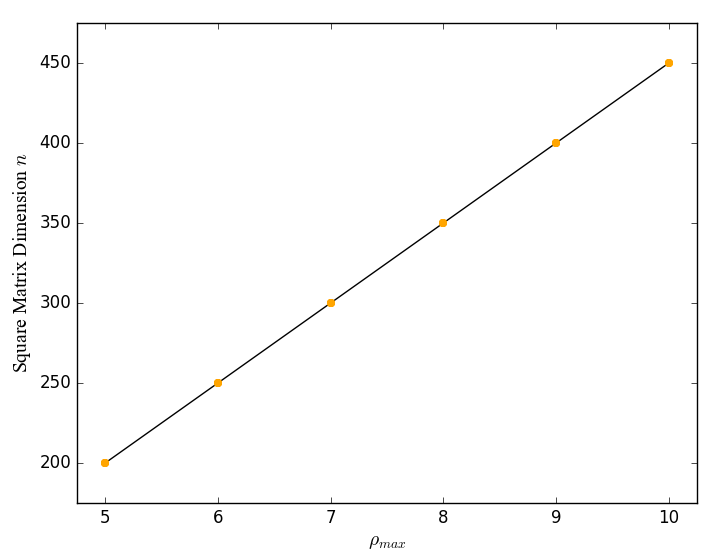
\includegraphics[width=0.7\textwidth]{Code/RhoDepend.png}\end{center}
		\end{frame}

		\begin{frame} \frametitle{Jacobi vs. Armadillo}
			The time needed to compute the lowest three eigenvalues for Jacobi's rotation algorithm and Armadillo's {\em eig\_sym} function were compared. The Armadillo library function was many orders of magnitude faster than the brute force Jacobi method.
		\end{frame}

		\begin{frame} \frametitle{Jacobi vs. Armadillo}
			\[
   		 	\begin{array}{c|ccc}
    		\toprule \midrule
    		\text{Dimensionality $n$} & \text{Eigenvalues} & t_\text{Armadillo} \text{ (s)} & t_\text{Jacobi} \text{ (s)} \\ \midrule
     		50   &  (2.99687, 6.98434, 10.9619)  &   0.000617    &    0.08572   \\ \midrule
    		100   &  (2.99922, 6.99609, 10.9907)  &    0.003777  &        1.15983   \\ \midrule
    		150  &   (2.99965, 6.99827, 10.9960)  &    0.007561    &      5.89020    \\ \midrule
     		200   &  (2.99980, 6.99903, 10.9978) &      0.012636       &  18.5741  \\ \midrule
    		250  &   (2.99988, 6.99938, 10.9987)   &    0.019315       &   49.3644   \\ \midrule
    		300  &   (2.99991, 6.99957, 10.9991)    &   0.032661  &        110.025   \\ \midrule
    		350  &   (2.99994, 6.99968, 10.9994)    &   0.061280     &     248.396     \\ \midrule
    		400  &   (2.99995, 6.99976, 10.9996)    &   0.086203     &     430.594    \\ \midrule
    		450  &   (2.99996, 6.99981, 10.9997)    &   0.094821  &        901.509    \\ \midrule
    		500  &   (2.99997, 6.99985, 10.9998)   &     0.123586   &       1394.52     \\ \midrule
    		\bottomrule
    		\end{array}
    		\]
		\end{frame}

		\begin{frame} \frametitle{Matrix Transformations}
			The transformations on the $n\times n$ matrix \textbf{A} grow as approximately $n^2$. 
			\begin{center}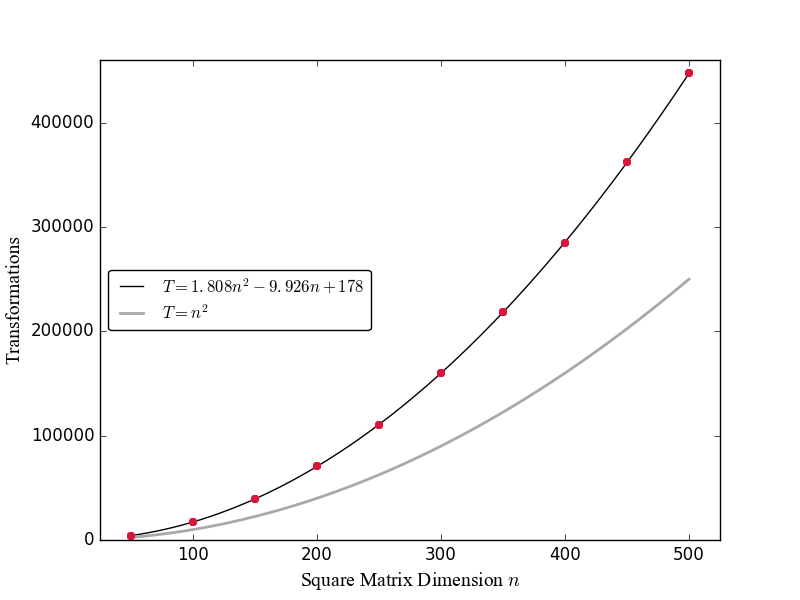
\includegraphics[width=0.7\textwidth]{Code/TvsN.png}\end{center}
		\end{frame}

		\begin{frame} \frametitle{2 Electron Wavefunctions}
			By varying the strength of the harmonic oscillator potential, the effect of coulombic interaction was observed.

			In the figures that follow, the strength of the oscillator potential is increased with each figure.

			The first figure has $\omega_r = 0.01$ \\
			The second figure has $\omega_r = 0.50$ \\
			The third figure has $\omega_r = 1.00$ \\
			The fourth figure has $\omega_r = 5.00$ 
		\end{frame}

		\begin{frame} \frametitle{2 Electron Wavefunctions}
			\begin{center}
    		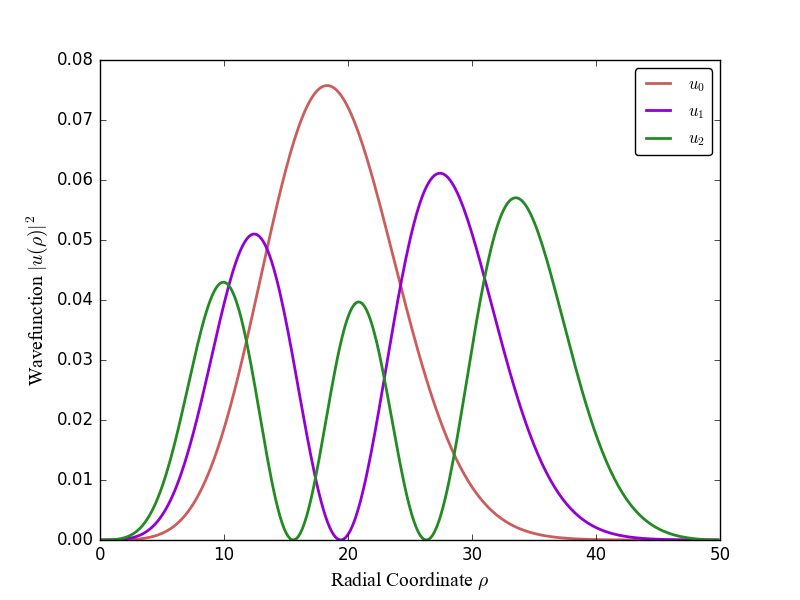
\includegraphics[width=.85\textwidth]{Code/WavefunctionOmega0p01.png}
    		\end{center}
		\end{frame}

		\begin{frame} \frametitle{2 Electron Wavefunctions}
			\begin{center}
    		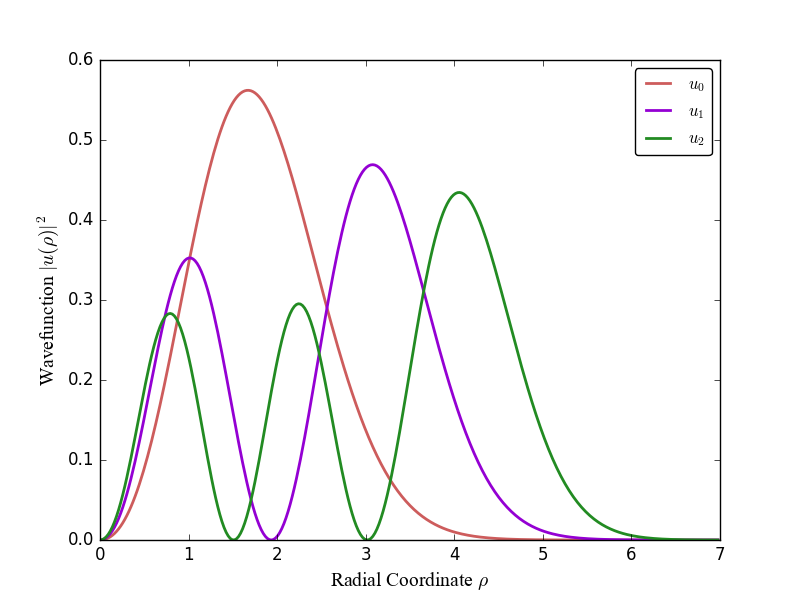
\includegraphics[width=.85\textwidth]{Code/WavefunctionOmega0p50.png}
    		\end{center}
		\end{frame}

		\begin{frame} \frametitle{2 Electron Wavefunctions}
			\begin{center}
    		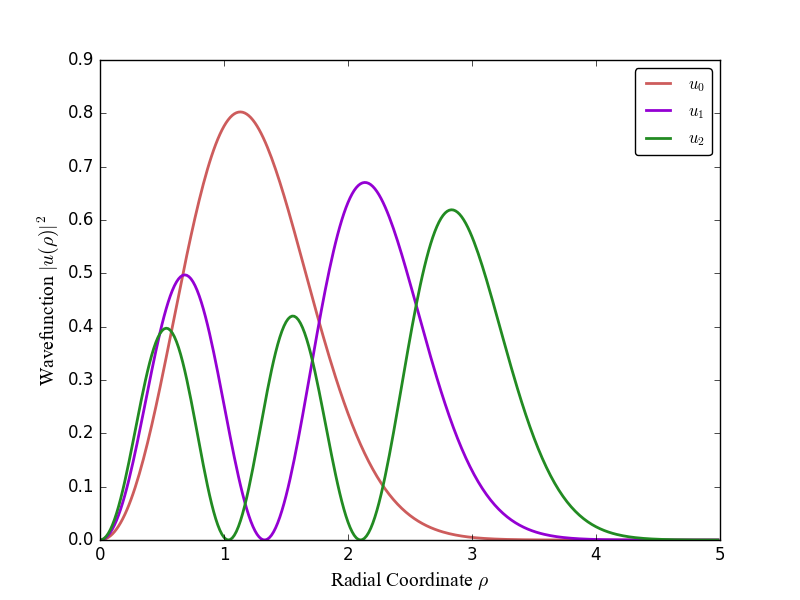
\includegraphics[width=.85\textwidth]{Code/WavefunctionOmega1.png}
    		\end{center}
		\end{frame}

		\begin{frame} \frametitle{2 Electron Wavefunctions}
			\begin{center}
    		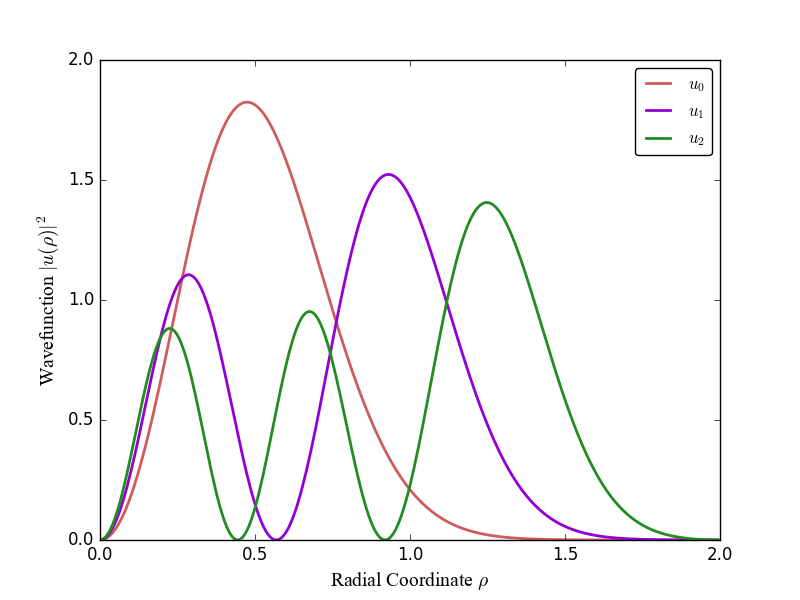
\includegraphics[width=.85\textwidth]{Code/WavefunctionOmega5.png}
    		\end{center}
		\end{frame}

	\section{Conclusions}
		\begin{frame} \frametitle{Summary}
			The first task was to impliment algorithms that solve a one electron system in a three dimensional harmonic oscilator potential well. To do this, a square matrix was diagonalized using both a brute-force Jacobi rotation algorithm and Armadillo. 
    		
		\end{frame}

		\begin{frame} \frametitle{Closing Thoughts}
			Jacobi's method for diagonalizing matrices was found to be orders of magnitude slower than the Armadillo library's {\em eig\_sym} function. This means that, while useful and simple to impliment, Jacobi's method is only practical for small matrices.

			If however, Armadillo is unavailable, Jacobi's method can be improved upon! (parallelization) 
			%maybe one processor per row or something
		\end{frame}

	\section{References}
		\begin{frame}
			\frametitle{Citations}
			\begin{thebibliography}{1}

			\bibitem{morten} 
    				M. Hjorth-Jensen, {\em Computational Physics}, University of Oslo (2015). 

			\bibitem{taut} M. Taut, Phys. Rev. A 48, 3561 - 3566 (1993).

			\bibitem{arma} C. Sanderson, {\em Armadillo}. {\bf 2010}. {\url arma.sourceforge.net}

			\end{thebibliography}
		\end{frame}

\end{document}